%!TeX root = Chapter_Results2
\documentclass[../../CompleteThesis2/Complete_2ndDraft]{subfiles}
%\graphicspath{{../../Figures/}}
\begin{document}

This chapter contains the final results of the stability tests presented in Chapter \ref{Chapter:Method} along with the final diffusion length estimates, based on the results of the stability tests and general considerations and observations made throughout the thesis. Finally these $\sigma$ estimates are used to give a first estimate of the temperature for the given depth interval.

\section[Annual Layer Thickness]{Annual Layer Thickness}
\label{Sec:Results_ALT}
The final annual layer thickness estimates are determined with a section length of $l_{\text{sec}}=7$ m and a shift of $l_{\text{shift}}=1.5$ m. From Table \ref{Tab:ALTEsts} it can be seen that $\lambda$ is smallest for Site E and Site G, which corresponds well with those sites having the lowest accumulation rates.

\begin{table}[ht]
	\centering
	\begin{tabular}{c|c|c|c|c|c}
		& Site A & Site B & Site D & Site E & Site G \\
		\hline
		\hline
		$\lambda$ [m] & $0.311 \pm 0.006$ & $0.326 \pm 0.008$ & $0.354 \pm 0.012$ & $0.246 \pm 0.005$ & $0.264 \pm 0.006$ \\
	\end{tabular}
	\caption[$\lambda_A$ Estimate at LT]{\small Annual Layer Thickness, $\lambda$, estimation at the depth between Laki and Tambora events.}
	\label{Tab:ALTEsts}
\end{table}



\section[Diffusion Lengths]{Diffusion Length Estimates}
\label{Sec:Results_DiffLenEst}
Before revealing the final $\sigma$ estimates, the results of the stability tests carried out are presented. This concerns the effects on the diffusion length by the different spectral transforms, the constant or variable $\sigma$, and using constraints or not. The results are presented with both the optimal found diffusion length, the afterwards corrected firn diffusion length and for some tests, the average run time for the algorithm.
%\subsection[AWI B-cores]{AWI B-cores}
%\label{Subsec:Results_DiffLenEst_AWIBcores}


%
%
%\begin{figure}[h]
%	\centering
%	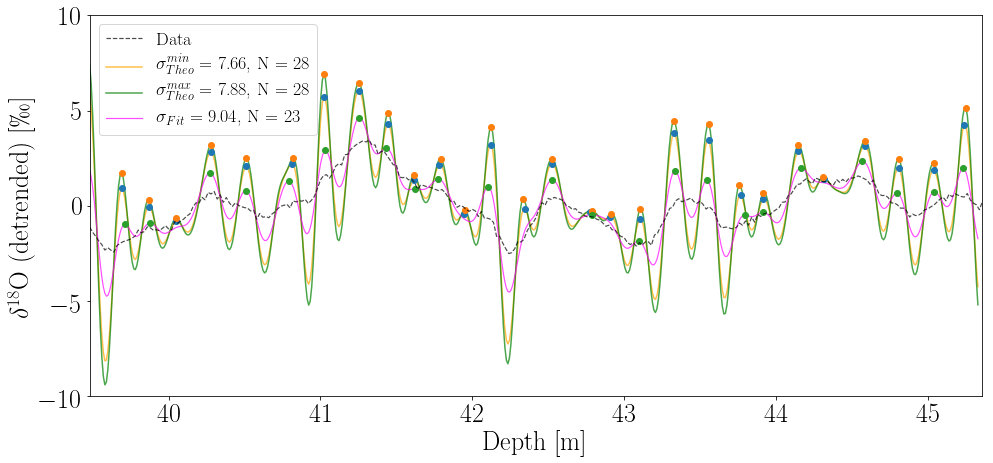
\includegraphics[width=0.8\textwidth]{B23_TheoDiffLens33Theo.png}
%	\caption[]{}
%	\label{fig:B23_BD_Theo}
%\end{figure}
%
%\begin{figure}[h]
%	\centering
%	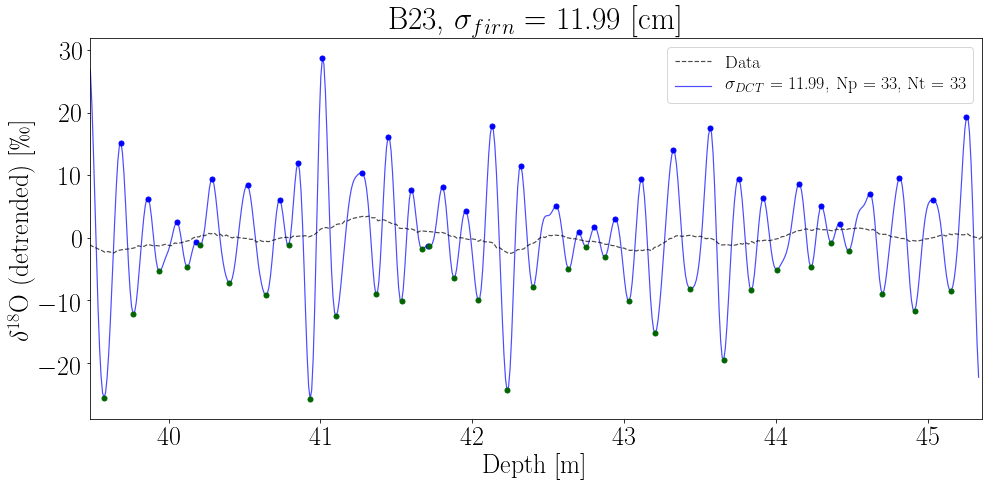
\includegraphics[width=0.8\textwidth]{B23_TheoDiffLens33Opt_only.png}
%	\caption[]{}
%	\label{fig:B23_BD_OptOnly}
%\end{figure}
%
%\begin{figure}[h]
%	\centering
%	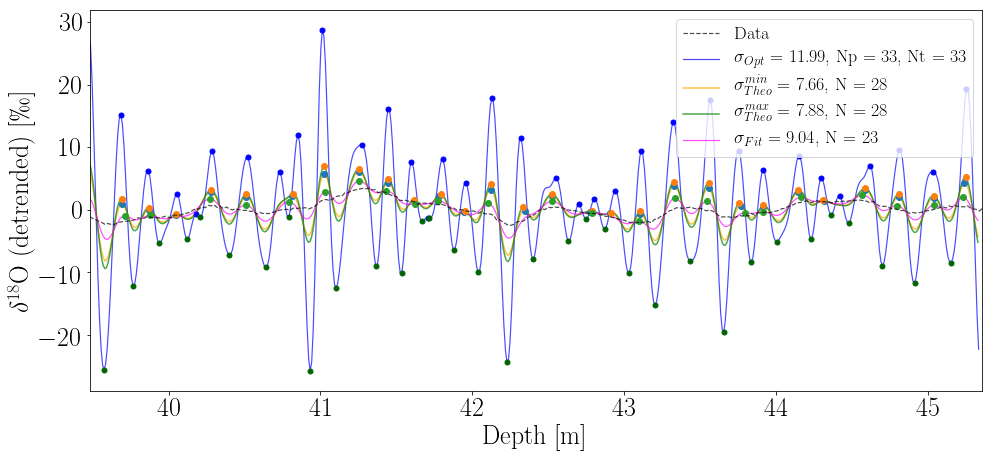
\includegraphics[width=0.8\textwidth]{B23_TheoDiffLens33OptBig.png}
%	\caption[]{}
%	\label{fig:B23_BD_OptBig}
%\end{figure}
%
%
%








%\subsection[Alphabet Cores]{Crete and Surrounding Alphabet Cores}
%\label{Subsec:Results_DiffLenEst_AlphabetCores}

\subsection[$\sigma$ Constraints or No constraints]{Diffusion Length Estimates if Constrained or Not Constrained}
\label{Subsec:Results_DiffLenEst_AlphabetCores_ConstraintsVNoConstraints}
The previous chapter presented the constrained method for optimization. The results of both constrained and unconstrained optimization can be seen in Table \ref{Tab:diffLens_ConstVNoConst}. If the method does not impose constraints on the algorithm, the algorithm is not quite as stable, as can be seen on the average run time and the run time variances. Furthermore, the unconstrained method systematically results in a diffusion length estimate lower than the one computed through the constrained method, and generally with a higher variance. 
\begin{table}[ht]
	\centering
	\begin{tabular}{l l l | c | c}
		& & & No Constraints & Constraints\\
		\hline
		\hline 
		\multirow{3}{*}{\textbf{Site A}} & $\sigma_{\text{opt}}$ & [cm] & $6.69 \pm 0.85$ & $7.88 \pm 0.66$\\
		& $\sigma_{\text{firn}}$ & [cm] & & \\
		& t & [s] & $19.85\pm 10.39$ & $8.84\pm 1.47$ \\
		\hline
		
		\multirow{3}{*}{\textbf{Site B}} & $\sigma_{\text{opt}}$ & [cm] & $5.98 \pm 0.24$ & $7.31 \pm 0.18$ \\
		& $\sigma_{\text{firn}}$ & [cm] & & \\
		& t & [s] & $11.66 \pm 4.46$ & $8.68 \pm 1.08$\\
		\hline
		
		\multirow{3}{*}{\textbf{Site D}} & $\sigma_{\text{opt}}$ & [cm] & $4.35 \pm 0.53$ & $6.94 \pm 0.24$ \\
		& $\sigma_{\text{firn}}$ & [cm] & & \\
		& t & [s] & $14.83\pm 8.50$& $9.19 \pm 0.72$\\
		\hline
		
		\multirow{3}{*}{\textbf{Site E}} & $\sigma_{\text{opt}}$ & [cm] & $6.20 \pm 0.20$ & $8.15 \pm 0.11$ \\
		& $\sigma_{\text{firn}}$ & [cm] & & \\
		& t & [s] & $5.44 \pm 1.82$ & $6.97 \pm 0.56$\\
		\hline
		
		\multirow{3}{*}{\textbf{Site G}} & $\sigma_{\text{opt}}$ & [cm] & $8.55 \pm 0.27$ & $9.35 \pm 0.26$ \\
		& $\sigma_{\text{firn}}$ & [cm] & & \\
		& t & [s] & $29.99 \pm 3.81$ & $7.19 \pm 0.48$\\
		
		\hline
	\end{tabular}
	\caption[$\sigma$ Estimates Given Unconstrained and Constrained Method]{\small Optimal and corrected firn diffusion length estimates with either the non-constrained or the constrained method.}
	\label{Tab:diffLens_ConstVNoConst}
\end{table}


\subsection[Diffusion Length V N Peaks]{Diffusion Length Estimates vs. Counted Peaks}
\label{Subsec:Results_DiffLenEst_AlphabetCores_DiffLenVPeaks}
To get an understanding of how the diffusion length affected the number of counted years, a run was made going through all diffusion lengths from 1 cm to 15 cm for all cores. Illustrations of the results can be seen in Figures \ref{fig:AllCores_NpeaksVDiffLen} and \ref{fig:AllCores_NpeaksVDiffLenZoom}. In Figure \ref{fig:AllCores_NpeaksVDiffLen} it can be seen that the number of counted peaks generally increases as the diffusion length increases, until some value where the counts starts being more irregular. 
When looking at Figure \ref{fig:AllCores_NpeaksVDiffLenZoom}, it can be seen that for most of the cores, there exists a stable plateau of diffusion lengths that all result in $N_P=33$, for some longer than for others. This could be used as a stability measure and a sanity check of the number of years assumed is actually likely in this section. 

\begin{marginfigure}
	\centering
	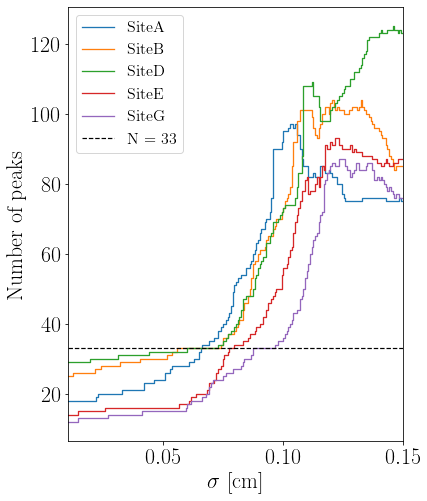
\includegraphics[width=\marginparwidth]{AllCores_NpeaksVDiffLen.png}
	\caption[$\sigma$ vs. N Peaks]{\footnotesize Number of peaks estimated given diffusion length, based on diffusion length in the interval [0.01; 0.15] m.}
	\label{fig:AllCores_NpeaksVDiffLen}
\end{marginfigure}

\begin{figure}[h]
	\centering
	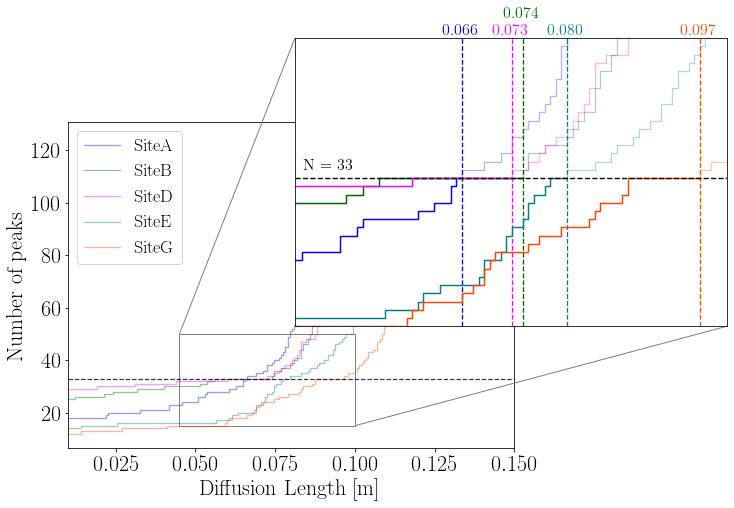
\includegraphics[width=0.8\textwidth]{AllCores_NpeaksVDiffLen_wZoom.png}
	\caption[$\sigma$ vs. N Peaks]{\small A zoom-in of the N peaks v. diffusion length plot in Figure \ref{fig:AllCores_NpeaksVDiffLen}. Specifically in focus are the maximal diffusion lengths corresponding to $N_{\text{peaks}}=33$.}
	\label{fig:AllCores_NpeaksVDiffLenZoom}
\end{figure}



\subsection[$\sigma$ v. Spectral Transforms]{Diffusion Length Estimates vs. Spectral Transform Methods}
\label{Subsec:Results_DiffLenEst_AlphabetCores_SpectralTransforms}
In Table \ref{Tab:DiffLens_SpecTrans} the estimated diffusion lengths, both optimal and firn, are presented along with the average run time of the method. The error is estimated through drawing the Laki and Tambora event locations from a Gaussian distribution with standard deviation of two months. For all sites, the results of all three methods are almost within each others margins. This might point to choosing one of the faster back diffusion methods to estimate the diffusion length with, if it is used for a quantitative measure. If it is needed to reconstruct a single data series one time, it might be preferable to use the NDCT.

\begin{table}[ht]
	\centering
	\begin{tabular}{l l l | c | c | c}
		& & & FFT & DCT & NDCT \\
		\hline
		\hline 
		\multirow{3}{*}{\textbf{Site A}} & $\sigma_{\text{opt}}$ & [cm] & $7.57 \pm 0.60$ & $7.80 \pm 0.68$ & $7.26 \pm 0.53$ \\
		& $\sigma_{\text{firn}}$ & [cm] & & & \\
		& $t$ & [s] & $8.00 \pm 0.91$ & $7.93 \pm 0.91$ & $17.46 \pm 0.98$ \\
		\hline
		
		\multirow{3}{*}{\textbf{Site B}} & $\sigma_{\text{opt}}$ & [cm] & $7.11 \pm 0.40$ & $7.30 \pm 0.20$ & $7.36 \pm 0.21$ \\
		& $\sigma_{\text{firn}}$ & [cm] & & & \\
		& $t$ & [s] & $8.64 \pm 0.51$ & $8.41 \pm 0.82$ & $19.06 \pm 0.55$ \\
		\hline
		
		\multirow{3}{*}{\textbf{Site D}} & $\sigma_{\text{opt}}$ & [cm] & $7.00 \pm 0.41$ & $6.96 \pm 0.28$ & $7.21 \pm 0.27$ \\
		& $\sigma_{\text{firn}}$ & [cm] & & & \\
		& $t$ & [s] & $9.24 \pm 0.73$ & $9.20 \pm 0.69$ & $19.55 \pm 1.03$ \\
		\hline
		
		\multirow{3}{*}{\textbf{Site E}} & $\sigma_{\text{opt}}$ & [cm] & $8.07 \pm 0.01$ & $8.15 \pm 0.11$ & $8.21 \pm 0.14$ \\
		& $\sigma_{\text{firn}}$ & [cm] & & & \\
		& $t$ & [s] & $7.28 \pm 0.36$ & $7.03 \pm 0.56$ & $16.61 \pm 0.54$ \\
		\hline
		
		\multirow{3}{*}{\textbf{Site G}} & $\sigma_{\text{opt}}$ & [cm] & $9.38 \pm 0.32$ & $9.35 \pm 0.25$ & $9.44 \pm 0.24$ \\
		& $\sigma_{\text{firn}}$ & [cm] & & & \\
		& $t$ & [s] & $7.53 \pm 0.49$ & $7.24 \pm 0.49$ & $16.45 \pm 0.34$ \\
		\hline
	\end{tabular}
	\caption[$\sigma$ Estimates Given Spectral Transforms]{\small Diffusion length estimates resulting in $N_{\text{peaks}}=33$ based on different spectral transform methods, namely the FFT, DCT and NDCT presented in earlier chapters and described in Appendix \ref{AppIV:SpectralTransforms}. Along with the optimal diffusion length, the actual firn diffusion length is presented - corrected for sampling diffusion, ice diffusion and thinning. The computational time of the back diffusion process given the different spectral transforms is also presented.}
	\label{Tab:DiffLens_SpecTrans}
\end{table}


\subsection[$\sigma$ Constant or Variable]{Diffusion Length Estimates if Diffusion Length Constant or Variable}
\label{Subsec:Results_DiffLenEst_AlphabetCores_SigConstVar}

\begin{table}[ht]
	\centering
	\begin{tabular}{l l l | c | c}
		& & & $\sigma_{\text{constant}}$ & $\sigma(z)$\\
		\hline
		\hline 
		\multirow{2}{*}{\textbf{Site A}} & $\sigma_{\text{opt}}$ & [cm] & $ \pm$ & $ \pm $\\
		& $\sigma_{\text{firn}}$ & [cm] & & \\
		\hline
		
		\multirow{2}{*}{\textbf{Site B}} & $\sigma_{\text{opt}}$ & [cm] & $ \pm $ & $ \pm $ \\
		& $\sigma_{\text{firn}}$ & [cm] & & \\
		\hline
		
		\multirow{2}{*}{\textbf{Site D}} & $\sigma_{\text{opt}}$ & [cm] & $ \pm $ & $ \pm $ \\
		& $\sigma_{\text{firn}}$ & [cm] & & \\
		\hline
		
		\multirow{2}{*}{\textbf{Site E}} & $\sigma_{\text{opt}}$ & [cm] & $ \pm $ & $ \pm $ \\
		& $\sigma_{\text{firn}}$ & [cm] & & \\
		\hline
		
		\multirow{2}{*}{\textbf{Site G}} & $\sigma_{\text{opt}}$ & [cm] & $ \pm $ & $ \pm $ \\
		& $\sigma_{\text{firn}}$ & [cm] & & \\
		
		\hline
	\end{tabular}
	\caption[$\sigma$ Given Constant or Varying]{\small Optimal and corrected firn diffusion length estimates given either a $\sigma$ estimated to be constant, $\sigma_{\text{constant}}$, or varying, $\sigma(z)$, over the Laki to Tambora depth section. }
\end{table}

%\begin{table}[ht]
%	\centering
%	\begin{tabular}{l||*{6}{c | c||}}
%		&
%		\multicolumn{2}{c}{Crete} & \multicolumn{2}{c}{Site A} & \multicolumn{2}{c}{Site B} & \multicolumn{2}{c}{Site D} & \multicolumn{2}{c}{Site E} & \multicolumn{2}{c||}{Site G} \\
%		%\hline
%		&
%		$\sigma_{\text{opt}}$ & $\sigma_{\text{firn}}$ & $\sigma_{\text{opt}}$ & $\sigma_{\text{firn}}$ & $\sigma_{\text{opt}}$ & $\sigma_{\text{firn}}$ & $\sigma_{\text{opt}}$ & $\sigma_{\text{firn}}$ & $\sigma_{\text{opt}}$ & $\sigma_{\text{firn}}$ & $\sigma_{\text{opt}}$ & $\sigma_{\text{firn}}$ \\
%		
%		\hline
%		$\sigma_{\text{constant}}$ & & & & & & & & & & & & \\ 
%		$\sigma(z)$ & & & & & & & & & & & & \\ 
%	\end{tabular}
%\end{table}

%\begin{figure}
%	\centering
%	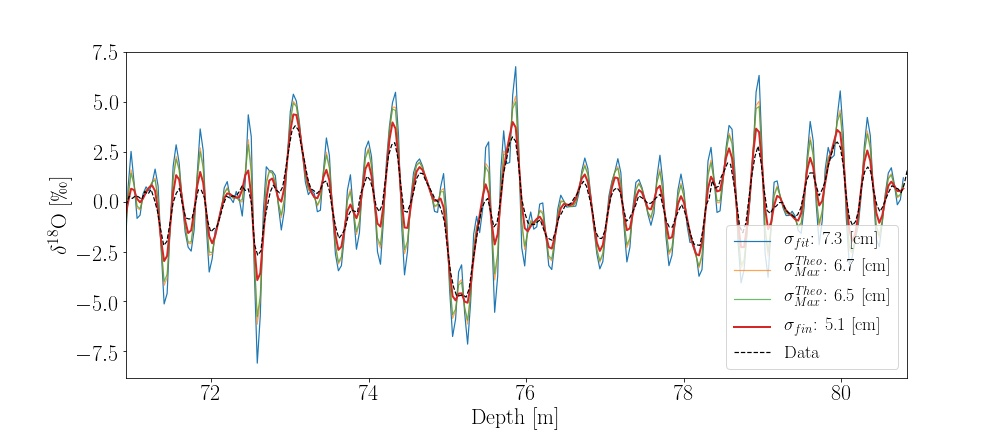
\includegraphics[width=\textwidth]{SiteA_BackDiffused_AllSigmaEst.jpg}
%	\caption[All diffusion length estimate deconvolutions, Site A]{Estimated back diffused data series with different diffusion length estimates: diffusion length estimate from spectral fit ($\sigma_{fit}$), maximum ($\sigma_{Max}^{Theo}$) and minimum ($\sigma_{Min}^{Theo}$) theoretically estimated diffusion lengths and final estimated diffusion length.}
%	\label{fig:SiteA_BackDiffused_AllSigmaEst}
%\end{figure}



\subsection[Final $\sigma$ Estimates]{Final $\sigma$ Estimates Based on Previous Conclusions}
\label{Subsec:Results_DiffLenEst_AlphabetCores_FinalEstimates}
The temperature estimates are, as described previously, made based on a steady state model, with a constant accumulation rate. The estimate is then made numerically through a Newton-Raphson scheme from \lstinline[language=Python]|scipy.optimize.newton|, finding the roots of $\sigma_{\text{model}}\cdot \frac{\rho_{\text{CO}}}{\rho_{\text{ice}}} - \sigma_{\text{data}}$.
The temperature estimates can be seen in Table \ref{Tab:TempEstStSt} and the underlying distributions in Figure \ref{fig:AllCores_StStTempEsts}. Again in these distributions can the quantization of the results be seen, resulting in non-Gaussian distributions.
\begin{table}[ht]
	\centering
	\begin{tabular}{l l l | c }
		& & & $\sigma_{\text{final}}$\\
		\hline
		\hline 
		\multirow{2}{*}{\textbf{Site A}} & $\sigma_{\text{opt}}$ & [cm] & $ \pm$ \\
		& $\sigma_{\text{firn}}$ & [cm] & \\
		\hline
		
		\multirow{2}{*}{\textbf{Site B}} & $\sigma_{\text{opt}}$ & [cm] & $ \pm $ \\
		& $\sigma_{\text{firn}}$ & [cm] & \\
		\hline
		
		\multirow{2}{*}{\textbf{Site D}} & $\sigma_{\text{opt}}$ & [cm] & $ \pm $ \\
		& $\sigma_{\text{firn}}$ & [cm] & \\
		\hline
		
		\multirow{2}{*}{\textbf{Site E}} & $\sigma_{\text{opt}}$ & [cm] & $ \pm $ \\
		& $\sigma_{\text{firn}}$ & [cm] & \\
		\hline
		
		\multirow{2}{*}{\textbf{Site G}} & $\sigma_{\text{opt}}$ & [cm] & $ \pm $ \\
		& $\sigma_{\text{firn}}$ & [cm] & \\
		
		\hline
	\end{tabular}
\caption[Final $\sigma$ Estimates]{\small Final diffusion length estimates, based on conclusions made previously in different tests.}
\label{Tab:TempEstStSt}
\end{table}






\section[Temperature Estimates from Data]{Final Temperature Estimates from Optimal Estimated $\sigma$}
\label{Sec:Results_TempEstData}

\todo{RES-DATAEST: Write entire section.}

\subsection[Steady State Solution]{Steady State Solution}
\label{Sec:Results_TempEstData_StSt}
\todo{RES-DATAESTSTST: Write entire section.}

\begin{table}[ht]
	\centering
	\begin{tabular}{l c|c|c|c|c|c}
		& & Site A & Site B & Site D & Site E & Site G \\
		\hline
		\hline
		$T_0$ & [$^{\text{o}}$C] & -29.41 & -29.77 & -28.3 & -30.37 & -30.1 \\
		$\bar{T}_{\text{StSt}}$ & [$^{\text{o}}$C] & $-31.04 \pm 2.02$ & $-30.46 \pm 0.83$ & $-30.00 \pm 1.05$ & $-30.89 \pm 0.48$ & $-25.97 \pm 0.70$ \\
	\end{tabular}
	\caption[Steady State Temperature Estimates]{\small Steady state temperature estimates based on the final firn diffusion length estimates found. $T_0$ is the temperature used to generate the theoretical diffusion length and density profiles, and originates from \cite[add. text]{keylist}}
\end{table}

\begin{figure}[h]
	\centering
	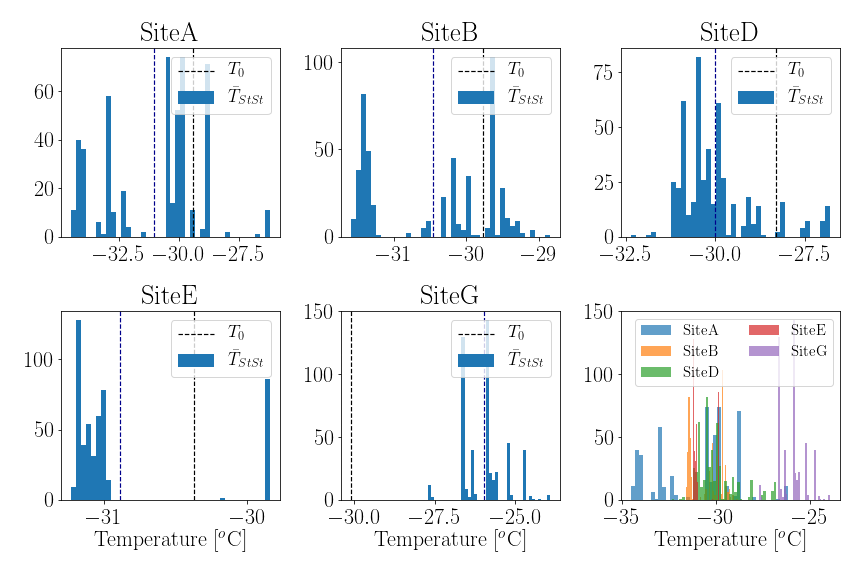
\includegraphics[width=0.9\textwidth]{AllCores_StStTempEsts.png}
	\caption[Steady State Temperature Distributions]{\small Steady State Temperature Distributions}
	\label{fig:AllCores_StStTempEsts}
\end{figure}



\subsubsection[Accumulation Distributions]{Accumulation Distributions}
\label{Sec:Results_TempEstData_StSt_AccumDists}
\todo{RES-DATAESTACCUM: Write entire section.}

\subsection[Iso-CFM Possibilities]{Further Possibilities of the Iso-CFM}
\label{Sec:Results_TempEstData_IsoCFMPossibilities}
\todo{RES-DATAESTCFM: Write entire section.}

\end{document}
